% Gemini theme
% https://github.com/anishathalye/gemini

\documentclass[final]{beamer}

% ====================
% Color options
% ====================

\newif\ifgrayhighlight % define new flag
% \grayhighlighttrue     % Use gray background for highlighted block
\grayhighlightfalse    % Use cardinal red background for highlighted block

% ====================
% Packages
% ====================

\usepackage[T1]{fontenc}
\usepackage{lmodern}
\usepackage[size=custom,width=120,height=120,scale=1.0]{beamerposter}
\usetheme{gemini}
\usecolortheme{stanford}
\usepackage{graphicx}
\usepackage{booktabs}
\usepackage{tikz}
\usepackage{pgfplots}
\pgfplotsset{compat=1.14}
\usepackage{anyfontsize}
\usepackage[numbers,super]{natbib}

% ====================
% Lengths
% ====================

% If you have N columns, choose \sepwidth and \colwidth such that
% (N+1)*\sepwidth + N*\colwidth = \paperwidth
\newlength{\sepwidth}
\newlength{\colwidth}
\setlength{\sepwidth}{0.025\paperwidth}
\setlength{\colwidth}{0.3\paperwidth}

\newcommand{\separatorcolumn}{\begin{column}{\sepwidth}\end{column}}

% ====================
% Title
% ====================

\title{Software Best Practices for Reproducible Open Science}

\author{Alex Koufos (he/him)\inst{1}} %\and Ben Bitdiddle \inst{1}}

\institute[shortinst]{\inst{1} Stanford University}

% ====================
% Footer (optional)
% ====================

\footercontent{
  \href{https://github.com/exoticdft}{https://github.com/exoticdft} \hfill
  TESS/SPD 2024 - Dallas, TX --- 211-040 \hfill
  \href{mailto:akoufos@sun.stanford.edu}{akoufos@sun.stanford.edu}
}
% (can be left out to remove footer)

% ====================
% Logo (optional)
% ====================

% use this to include logos on the left and/or right side of the header:
\logoleft{
\includegraphics[height=3cm]{logos/stanford+solar_group+HEPL-white.pdf}}
\logoright{
\includegraphics[height=7cm]{logos/SUTree-2color.pdf}}

% ====================
% Body
% ====================

\begin{document}

\begin{frame}[t]
\begin{columns}[t]
\separatorcolumn

\begin{column}{\colwidth}

  \begin{block}{Is there a "reproducibility crisis" in the sciences?}

    Over the past two decades, many researchers from several science communities
    have been discussing a potential issue related to the ability to reproduce
    scientific work.
    This issue has been termed the "Reproducibility Crisis" in the sciences.
    The 2016 Nature article\cite{baker2016} discusses this crisis in detail.
       
    \begin{figure}
      \centering
      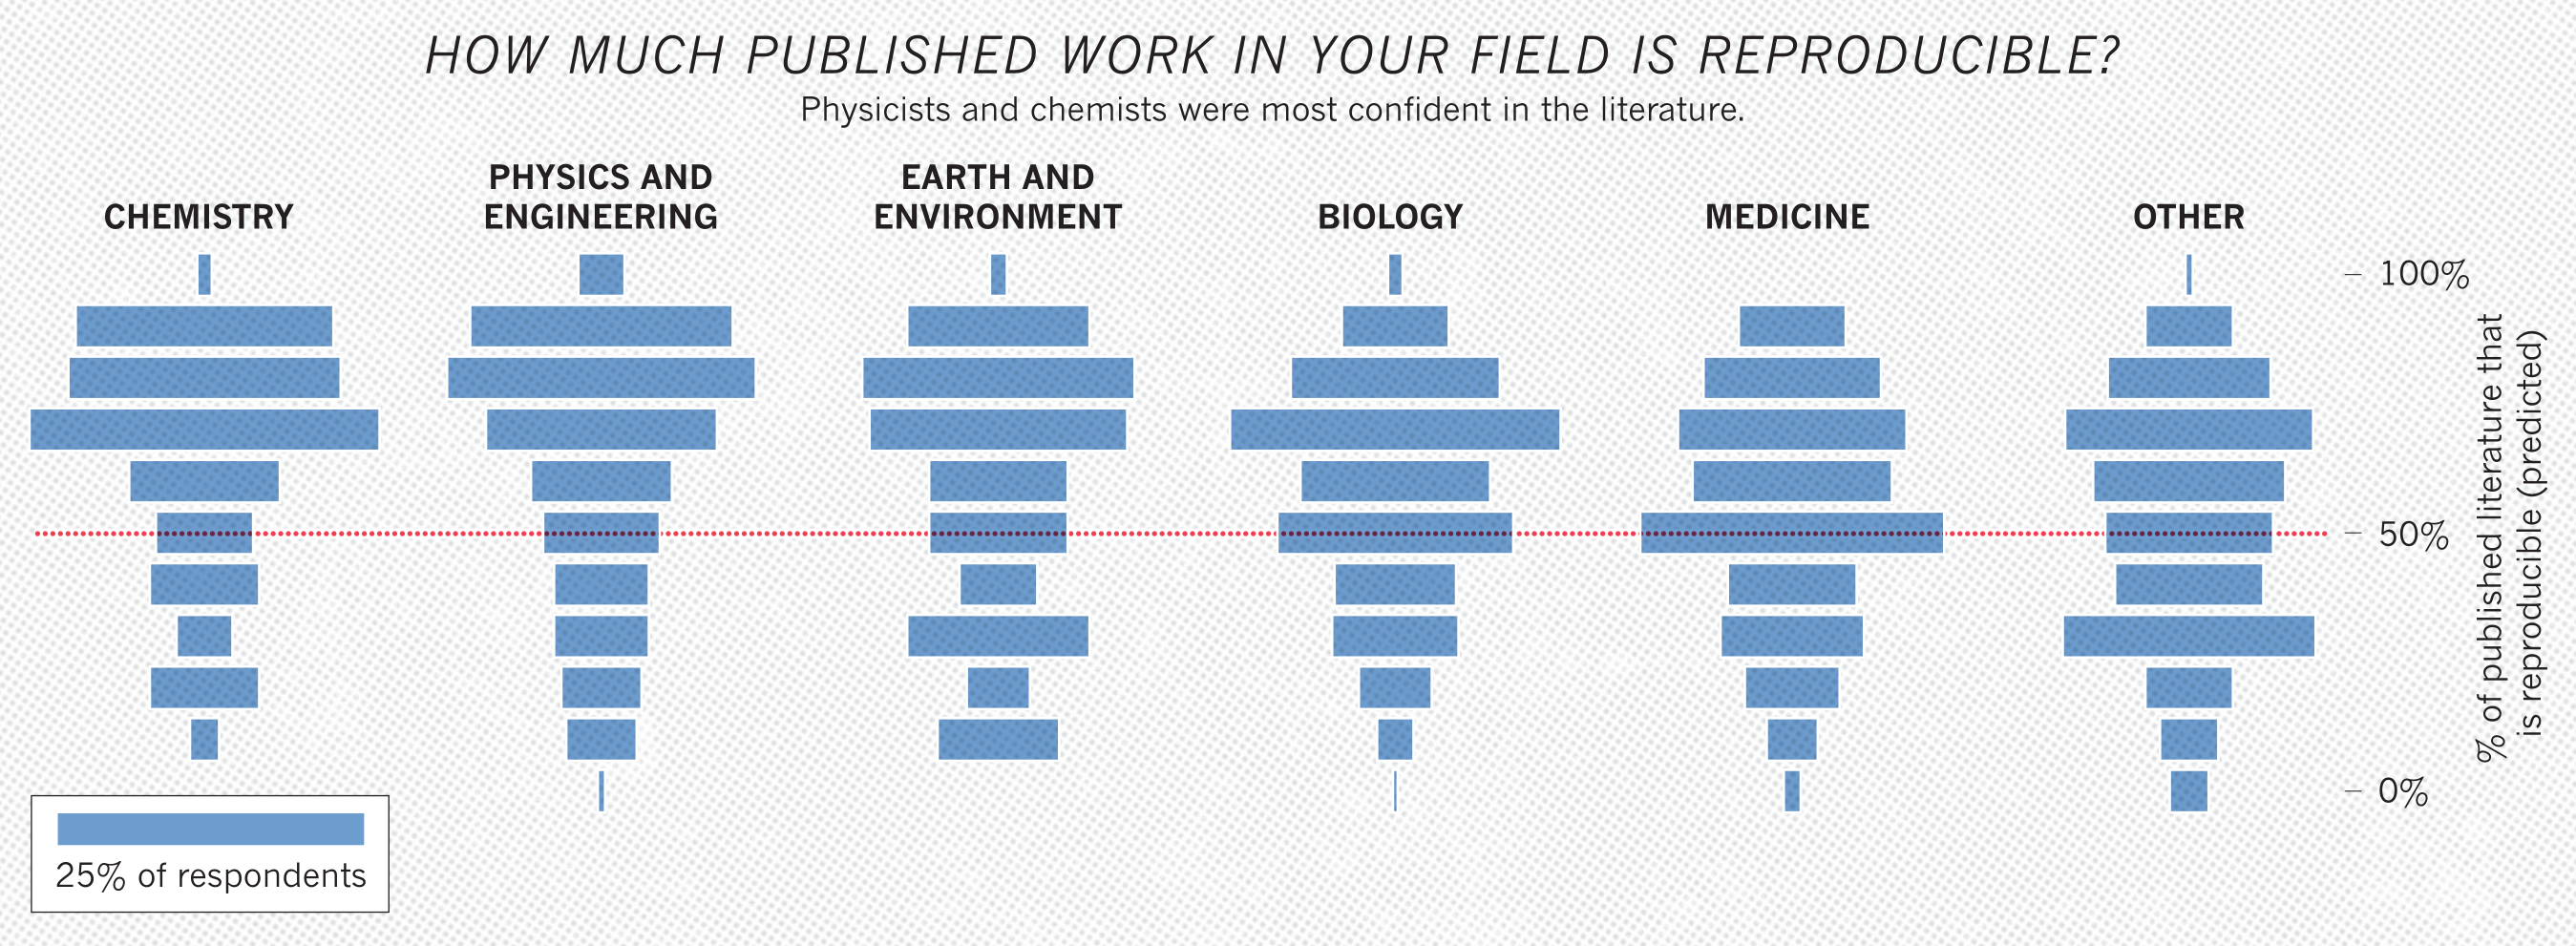
\includegraphics[width=0.85\textwidth]{tess2024/Nature-Field-Confidence.png}
      \caption{Science Field Based Confidence in Published Work (Baker, M. 2016)\cite{baker2016}}
      \label{fig:confidence}
    \end{figure}

    Figure~\ref*{fig:confidence} shows the general expectation of reproducible
    work within the various scientific communities.
    In general, the physics and engineering community has a higher confident in
    published literature.
    For example, nearly half of the respondents from physics and
    engineering fields were confident at least $80\%$ of the research could be
    reproduced.
    Note, however, that there are still many researchers who were not confident.
    This certainly doesn't help with the general public's confidence in modern
    scientific research.

    \begin{figure}
      \centering
      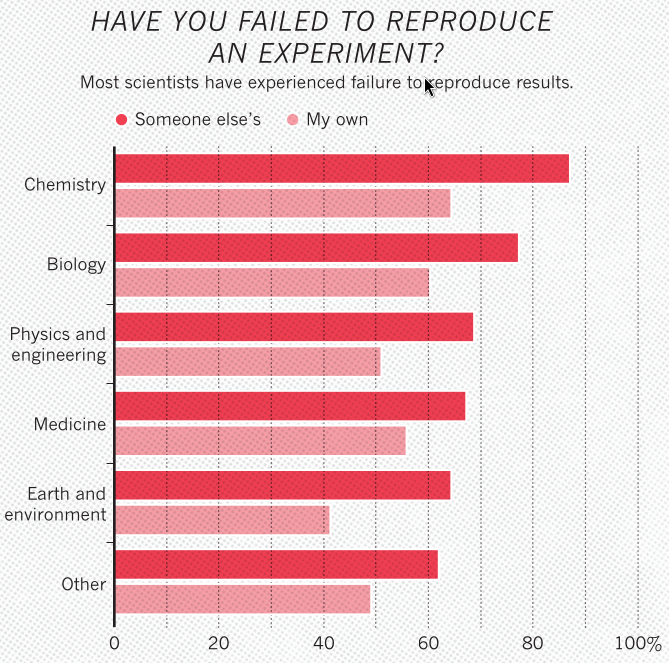
\includegraphics[width=0.85\textwidth]{tess2024/Nature-Reproducibility-Failure-.png}
      \caption{Failure to Reproduce Published Results (Baker, M. 2016)\cite{baker2016}.
      Higher values represent greater failure in reproducing experiments.}
      \label{fig:failure}
    \end{figure}
    
    Figure~\ref*{fig:failure} presents the failure researchers had when trying
    to reproduce experiments within the their fields.
    The results shown suggest a significant issue in all fields, and show an
    obvious conflict from the expections in Figure~\ref*{fig:confidence}.
    In all research communities, researchers struggled to reproduce the results
    of others, and even themselves.

  \end{block}

  \begin{alertblock}{A Failure to Reproduce}
    Several reports have suggested there is a problem with researchers being
    able to reproduce their own work.
    Baker's research\cite{baker2016} suggests \textbf{over 50\% of the physics
    and engineering community were unable to reproduce their own work!}

  \end{alertblock}

  \begin{block}{But what is Reproducibility?}
    The National Academies of Sciences, Engineering, and Medicine was asked to
    conduct a study assessing how prevalent the issues related to
    reproducibility and replicability and offer recommendations for improving
    transparency and rigor in scientific research.
    A committee was from and in 2019 they released their
    report\cite{reproducibility_in_science}.
    Within they define
    \begin{description}
      \item[reproducibility (i.e. computational reproducibility)] \hfill \\
      as obtaining consistent computational results using the same input data,
      computational steps, methods, code, and conditions of analysis
      \item[replicability] \hfill \\
      as obtaining consistent results across studies aimed at answering the same
      scientific question, each of which has obtained its own data
    \end{description}

    This poster will focus on the former definition, as well as other related
    goals for software.
    There are many techniques we can all use to help alleviate potential issues
    with being able to reproduce results.

  \end{block}

\end{column}

\separatorcolumn

\begin{column}{\colwidth}

  \begin{exampleblock}{Ways to help mitigate reproducibility issues in your research}

    Software is essential and inherit in every aspect of modern research.
    The coding we do for this research is often considered a means to an end 
    and ignored for what it is; software engineering.
    However, we can learn a lot from the software engineering community and
    in the recent years there has been an emergence of associations focused on 
    "research software engineering (RSEng)", specifically.
    One such organization is the
    \href{https://us-rse.org}{United States Research Software Engineer Association (US-RSE)}
    \cite{us-rse} (several others are mentioned in the references section.)
    These communities strive to promote scientific software best practices to
    support better research.
    For example, the Better Scientific Software (BSSw)\cite{bssw} provides many
    resources, such as
    \href{https://bssw.io/items?topic=reproducibility}{https://bssw.io/items},
    to help researchers and RSEs create successful research projects.

    Although these resources can be extremely useful, there are a large amount
    of "best practices" one can use, which can get overwhelming quickly.
    Below I discuss some of the "easier" and possibly more impactful tools one
    can use.
    This poster will focus on \textbf{version control}, \textbf{code reviews},
    and \textbf{documentation}.
    
    Focusing some effort on these best practices can help with the goals of:
    \begin{itemize}
      \item Higher \textbf{reusability} of code (less need to copy and paste
        things that already work)
      \item Better \textbf{reproducibility} and \textbf{robustness} of software
        (verify/validate results and handle errors)
      \item Improved \textbf{scalability} (ability to add new features and
        complexity)
      \item Enhanced \textbf{collaboration} (work with others)
      \item Boosted \textbf{clarity} (reminders of what you did and helps other
        follow)
      \item Greater \textbf{transferability} of data and programs (work
        anywhere, sharing, etc.)
      \item \textbf{Transparency} of results and methods (helps public trust
        and explaining to others)
    \end{itemize}
    
    \textbf{Disclaimer:} None of the these techniques can single handedly
    resolve, or entirely mitigate the problem of reproducibility.
    However, when implemented in tandem, can mitigate unforeseen challenges in
    future efforts to reproduce your work, both by others and yourself.

  \end{exampleblock}

  \begin{block}{Best Practice: Version Control}

    \heading{What is version control?}
    Version control is essentially a history of snapshots of your software.
    If you are unfamiliar with version control, you may have inadvertently used
    some system yourself for tracking your changes.
    For example,
    \href{https://phdcomics.com/comics/archive.php?comicid=1531}{PhD Comics}\cite{phdcomics}
    jokes about a common practice many of us (myself included) have used in the
    past to track our research papers, where you simply save a new file with
    changes from the last iteration and name it `whatever-rev2.doc`.
    This of course can get quite tenuous quickly when you have more than a few
    revisions.
    \\ \vspace{0.5em}
    \textbf{Protip:} Check out \href{overleaf.com}{overleaf.com} for tracking
    document changes if working with LaTeX.
    \\ \vspace{0.5em}
    This history of these changes (and all its metadata) is called a
    "repository" or "repo".

    \heading{Why use version control?}
    Version control can be an extremely useful tool to track changes to your
    software (and experimentation) throughout your research endeavor.
    It can help with \textbf{reproducibility}, \textbf{robustness},
    \textbf{scalability}, \textbf{collaboration}, and \textbf{transparency}.

    \heading{How you can use version control}
    When working with software, \href{https://git-scm.com/}{Git} is one of the
    most popular tools for version control.
    It ties directly into management software, such as
    \href{https://github.com}{GitHub} and \href{https://gitlab.com}{GitLab}.
    This is done by saving just the changes between snapshots as "commits" in
    a linked list, often visualized as a directional acyclic graph.
    Figure~\ref{fig:git-simple} and \ref{fig:git-github-flow} show the history
    of two different Git repositories.
    These type of diagrams are general known as "commit graphs".
    
    In both these figures, commits are shown as circles, with directional lines
    referencing a previous commit, like nodes in a linked list.
    Each commit contains the changes since the last commit (its parent node),
    thus tracking the history of the repo over time.
    This allows us to easily understand and compare changes between versions.
    People like to refer to these commit graphs like trees, with a trunk and
    branches off the trunk.

    \begin{figure}
      \centering
      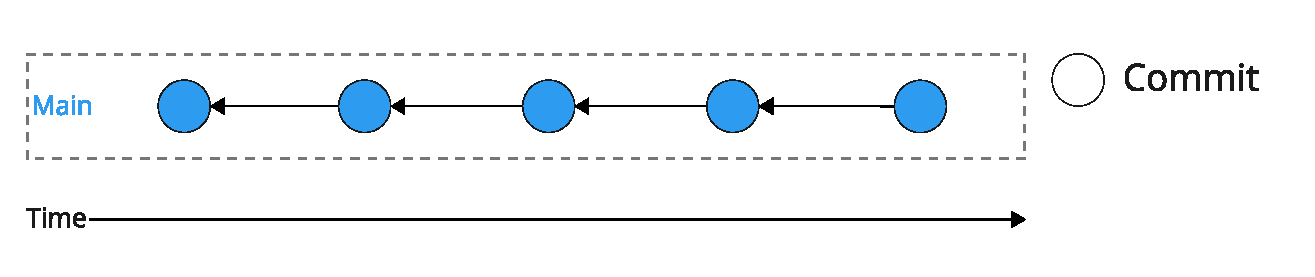
\includegraphics[width=0.95\textwidth]{tess2024/git-simple-git-repo.pdf}
      \caption{Version Control: A simple Git history of the "main" branch}
      \label{fig:git-simple}
    \end{figure}

    Figure~\ref*{fig:git-simple} shows the simplest way to use Git.
    In the figure we see just 5 commits starting from the left to the right.
    Each commit represents a snapshot of the repo at that moment in time,
    compared against the previous commit (the very first commit or snapshot
    is considered empty.)
    So, in this commit graph, we are simply committing each of our changes
    against the "main" branch, i.e. the trunk.

    \begin{figure}
      \centering
      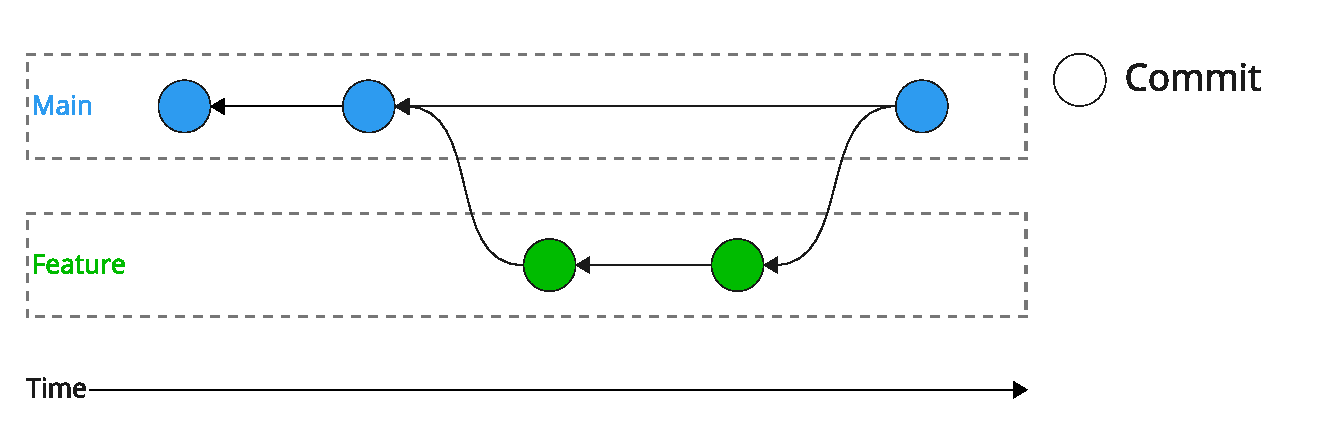
\includegraphics[width=0.95\textwidth]{tess2024/git-github-flow.pdf}
      \caption{Version Control: A Git repo using a branching model known as
        GitHub Flow}
      \label{fig:git-github-flow}
    \end{figure}

    Figure~\ref*{fig:git-github-flow} shows a slightly more involved way of
    tracking changes known as the "GitHub Flow" workflow, also called a
    "branching model".
    A branching model is simply a plan for managing and tracking your changes
    over time.
    Here the "main" branch or trunk is generally considered a stable branch;
    meaning the branch will attempt to only contain working, verified software,
    while the branches off of this trunk are a "work in progress" set of
    changes.
    These branches can be used as a way to iterate without protentially
    disrupting working software.
    When working as a team, they can also be used as a way for people to work on
    different parts of the software without necessarily stepping on each other.
    If you are interested in learning more about version control,
    \href{https://www.atlassian.com/git/tutorials/}{Atlassian}\cite{atlassian}
    offers many tutorials about Git.
    
    % Let's consider a really basic example of using this model.
    % One could imagine a code base with a script that prints some message, let's
    % say "Hello world!", to the screen.
    % The first commit, i.e. "initial commit", is just this simple script with
    % the functionality to print your message.
    % You add to the script an addition part of the message "Have a wonderful
    % day!" and commit this change to the main branch.
    % Now, you want to add new functionality (or feature) to your script to get
    % the name of the person calling your script.
    % Instead of committing directly to the main branch, which you know works, you
    % can make a branch off of main and begin adding your changes.
    % On this new branch, let's call it "feature", you add the ability to get user
    % input and update the message to "Hello World! Have a wonderful day,
    % \textit{User}!", then you commit on this new branch.
    % However, after making your commit, you realize there is an issue where the
    % user can provide anything as input, so you refine the input request to be
    % more specific and commit this change.
    % Once you are satisfied the new functionality is doing what you desire, you
    % finalize this branch by "merging" the changes back into the main branch.
    % Now, your main branches history will see these two commits as a single
    % set of changes against its previous stable commit.
    % In other words, the main branch will seem to have three commits in its
    % history all which work in a stable way.

  \end{block}

\end{column}

\separatorcolumn

\begin{column}{\colwidth}

  \begin{block}{Best Practice: Code Reviews}

    \heading{What are code reviews?}
    Code reviewing, simply put, is a process in which you, or others, look over
    the changes to your code (or repo) between two points in time.
    Essentially, having a second look at code changes.
    Generally, this is done at the end of (but sometimes during) a specific set
    of changes to the code base.
    These sets of changes are usually associated with a request for new
    functionality, resolving a known bug, updating existing functionality, or
    really anything you'd like.
  
    \heading{Why use code reviews?}
    Incorporating this process can be really helpful to catch bugs before they
    are added to stable code, or just used as a way to share how software works
    with team members.
    Code reviews can help with \textbf{reproducibility},
    \textbf{robustness},  \textbf{collaboration}, \textbf{clarity}, and 
    \textbf{transferability}.
  
    \heading{How you can use code reviews}
    Code review is one of the more involved processes, as it requires not only
    tools, but a standardize procedure to try to follow.
    And if working with others, interpersonal skills for relaying constructive
    comments when requesting changes based on your review.
    For each team, this procedure will likely be different.
    However, there are several resources you can reference to learn more.
    Here I briefly talk about the use of a process known as "pull requests" or
    "merge requests".
    This process is generally directly implemented by repo management tools I
    mentioned earlier, such as GitHub and GitLab.
    In general, the process is three or four steps:
    1. Update your codes (i.e. make changes),
    2. Use a tool to review differences from the initial snapshot of the codes
    (i.e. review changes),
    3. If neccessary, make suggestions and comments (discuss changes) and
    repeat the process, and finally
    4. Merge changes into stable code.
    Figure~\ref*{fig:code-review} shows the flow diagram of this process, with
    the option of discussing changes when the initial code changes might not be
    adequate.

    \begin{figure}
      \centering
      \vspace{-1em}
      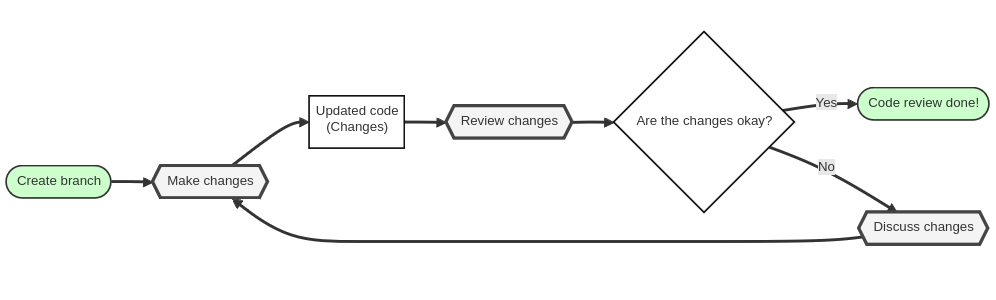
\includegraphics[width=0.95\textwidth]{tess2024/code-review-flow-diagram.png}
      \caption{Code Review: The basic code review process}
      \label{fig:code-review}
    \end{figure}
    
    GitHub has a built-in system for doing these code reviews.
    However, you can implement the process without it; GitHub and GitLab, just
    make it easier.
    You will need to learn a bit of GitHub to do the process, but you'd have to
    do the same if you implement your own process.
    If you decide to use GitHub, there are many useful resouces online to learn
    and practice the process before implementing on an important codebase.
    For example, an interactive tutorial can be found at
    \href{https://code-review.org}{code-review.org}\cite{code-review}.

  \end{block}

  \begin{block}{Best Practice: Documentation}

    \heading{What is documentation?}
    I think we all know this one.
    Documentation is simply the process of explaining the functionality and use
    of your software via some text-based system.

    \heading{Why use documentaiton?}
    This can be one of the most effective ways to onboard people or even just
    remind yourself of how your software works.
    How often have you written some software, thinking you won't need it again,
    only to pick it up again months or years later and asking yourself "What was
    I trying to do here?"; I know I have!
    Documentation can help with \textbf{reproducibility},
    \textbf{collaboration}, \textbf{clarity}, \textbf{transferability}, and
    \textbf{transparency}.

    \heading{How you can use documentation}
    As mentioned, documentation can be a great tool to remind yourself of how
    your software is supposed to work.
    Documentation can come in many forms.
    You can write documentation directly in the source code itself or at a
    higher level outside the source itself.
    For the former, you can use things like
    \href{https://realpython.com/documenting-python-code/}{docstrings} for
    Python and \href{https://www.doxygen.nl/manual/docblocks.html}{doxygen} for
    C/C++ or Fortran source code.
    The latter can be done by simply adding documents you can edit directly
    with your source code, like a .doc or .md file.
    Many of the repo management tools integrate Markdown (.md) or RestructedText
    (.rst) files directly in their systems.
    For example, you simple add a README.md file to the root of your repo, and
    GitHub/GitLab will directly create a nicely formatted document on the
    landing page of your repo.
    This README.md file is a great option as it is generally very humanreadable
    in plain text, making it easy to edit when you're working with your code.
    \\ \vspace{0.5em}
    \textbf{Protip:} Make documentation part of your pre code review process.
    Before submitting code to review, spend a few minutes updating any
    documentation related to your changes.
    \\ \vspace{0.5em}

  \end{block}

  \begin{block}{Best Practice: Others to consider}

    Some other best practices not covered here to consider is \textbf{testing},
    \textbf{Continuous Integration and Continuous Delivery (CI/CD)} or simply
    \textbf{automation}, and \textbf{issue tracking} to name a few.
    \textbf{Testing} helps with verifying results when you update software.
    \textbf{CI/CD} can help you automate some of the checks you may already be
    doing.
    Use \textbf{issue tracking} to track bugs in your software, converse about
    a specific issue, monitor future tasks, and prioritizing things related to
    your research.
    % I would also suggest looking at the concept of Kanban boards, if you like
    % to organize and track tasks.
    % As mentioned earlier, there are many resources provided by
    % US-RSE\cite{us-rse}, Society of Reseach Software Engineers\cite{uk-rse},
    % BSSw\cite{bssw}, Atlassian\cite{atlassian}, and many others.
    If interested in having a conversation, I suggest joining the US-RSE, it's
    free; or reach out directly.
    % You can also reach out to me directly at email below, or even on GitHub.

  \end{block}

  \begin{block}{References}

    \nocite{*}
    \footnotesize{\bibliographystyle{plainnat}\bibliography{poster}}

  \end{block}

\end{column}

\separatorcolumn
\end{columns}
\end{frame}

\end{document}
